\documentclass[12pt,a4paper]{report}
\usepackage{graphicx}
\usepackage{caption}
\usepackage{amsmath}
\usepackage{geometry}
\usepackage{listings}
 \geometry{
 a4paper,
 top=20mm,
 }
\usepackage[pdftex]{hyperref}
\usepackage{float}
\usepackage{titlesec}
\usepackage[utf8]{inputenc}
\usepackage[portuges]{babel}
\titleformat{\chapter}{\normalfont\huge}{\thechapter.}{10pt}{\huge\it} 
\begin{document}
\begin{titlepage}
	\centering
	
\includegraphics[width=0.3\textwidth]{uminho.jpg}\par\vspace{1cm}
	{\huge\bfseries Programação Orientada a Objetos \par}
	\vspace{0.5cm}
	{\scshape\ MIEI - 2º ano - 2º semestre\par}
	\vspace{0.1cm}
	{\scshape\ Universidade do Minho\par}
	\vspace{1.5cm}
    {\scshape\Huge\bfseries UMeR \par}
	\vspace{3cm}
	{\scshape\Huge\bfseries Grupo 29 \par}
    \vspace{1cm}
	{\scshape\ Frederico Pinto \par} 	\vspace{0.1cm}
	{\scshape\ A73639 \par}  \vspace{0.3cm}
	{\scshape\ José Sousa \par} \vspace{0.1cm}
	{\scshape\ A74678 \par}  \vspace{0.3cm}
	{\scshape\ Rui Vieira \par} \vspace{0.1cm}
	{\scshape\ A74658 \par}  \vspace{0.3cm}

	\vfill
	{\large \today\par}
\end{titlepage}

\tableofcontents

\chapter{Introdução}

Este projeto foi nos solicitado pelos docentes da UC \emph{Programação Orientada a Objetos}, onde nos foi proposta a realização de uma aplicação capaz de dar suporte a toda a funcionalidade que permita que um utilizador realize a viagem num táxi na empresa UMeR. Existem dois tipos de atores nesta aplicação, Cliente e Motorista. Os Clientes podem requisitar uma viagem, avaliar o motorista e consultar o seu histórico de viagens. Já os Motoristas só pode fazer a ultima do ator Cliente no entanto têm a possibilidade de adicionar um novo táxi, associar a si um táxi, registar uma viagem, sinalizar disponibilidade e associar-se a uma empresa tendo desta forma acesso á listagem de motoristas e táxis dessa mesma empresa podendo também desassociar-se da respetiva empresa.  

A realização deste projeto tinha como principal objetivo implementar em java os conhecimentos adquiridos na respetiva UC, em enfase para \emph{modularidade} e \emph{encapsulamento de dados} que até então não tinham sido abordadas ao longo nosso percurso académico.

\chapter{Descrição da aplicação}

Esta é uma aplicação com uma interface muito simples, de forma a que o utilizador possa tirar o maior proveito. Todos os menus funcionam à base de opções por números. 
Quando a aplicação é iniciada, o primeiro menu a que está sujeito o utilizador é o seguinte:


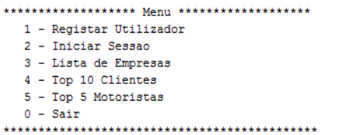
\includegraphics[width=0.7\linewidth, height=5cm]{1.png}

Neste menu, menu inicial, o utilizador pode registar-se, (Opção 1), e caso já o tenha feito pode iniciar sessão na Opção 2. Para além disso, ao escolher a Opção 3, o utilizador tem acesso à lista de Empresas existentes na aplicação. Ao escolher a Opção 4 ou Opção 5, o utilizador tem acesso ao Top 10 Clientes que mais gastam e ao Top 5 motoristas que apresentam mais desvios entre os valores previstos para as viagens e o valor final faturado. 


Se o utilizador decidir efetuar o registo será apresentado o seguinte menu:

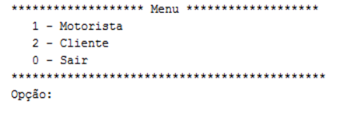
\includegraphics[width=0.7\linewidth, height=5cm]{2.png}

Após a apresentação deste menu, o utilizador pode escolher em registar-se como Motorista (Opção 1) ou Cliente (Opção2). Para isso terá de inserir determinadas informações necessárias para o registo: 

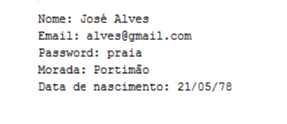
\includegraphics[width=0.7\linewidth, height=5cm]{3.png}

Depois do registo o utilizador pode agora iniciar sessão e desfrutar da aplicação. Depois de iniciar sessão será apresentado um menu consoante o tipo de utilizador que é, caso seja um Motorista, o seguinte menu é apresentado: 

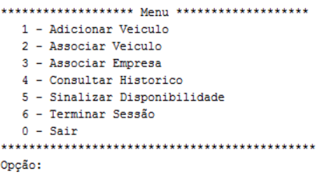
\includegraphics[width=0.7\linewidth, height=5cm]{4.png}

Opção 1 –  Esta opção permite ao utilizador (Motorista), registar uma viatura na aplicação.

Opção 2 – Permite ao utilizador associar uma viatura a si próprio.

Opção 3 -  Permite ao utilizador associar-se a uma empresa caso ela exista.

Opção 4 -  Com esta opção o utilizador pode consultar o seu histórico de viagens.

Opção 5 -  Nesta opção o utilizador (Motorista) pode mudar a sua disponibilidade. 

Opção 6 -  O utilizador termina sessão na aplicação.

Opção 0  - Volta atrás no menu.  

Caso o Motorista, escolha a Opção 3 e esta seja efetuada com sucesso, o Motorista passará a ser um Motorista de uma empresa e terá acesso a outro menu diferente: 

Opção 1 (Adicionar Veiculo) – Esta opção permite ao utilizador (Motorista), registar uma viatura na aplicação.

Opção 2 (Associar Veiculo) - Permite ao utilizador associar uma viatura a si próprio.

Opção 3 (Consultar Histórico) - Com esta opção o utilizador pode consultar o seu histórico de   viagens.

Opção 4 (Lista de Motoristas da Empresa) – Nesta opção é apresentada a lista de motoristas associados à empresa.

Opção 5 (Lista de Viaturas duma Empresa) – Nesta opção é apresentada a lista de viaturas associadas à empresa.

Opção 6 (Sinalizar Disponibilidade) - Nesta opção o utilizador (Motorista) pode mudar a sua disponibilidade.

Opção 7 (Desassociar Empresa) – Nesta opção o utilizador desassocia-se da empresa a que está ligado.

Opção 8 (Terminar Sessão) – O utilizador termina sessão na aplicação.

Opção 0  - Volta atrás no menu.  

No entanto, caso o utilizador seja um Cliente o menu apresentado é o seguinte: 

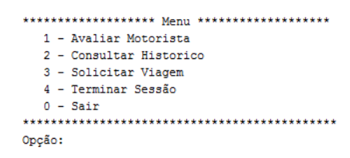
\includegraphics[width=0.7\linewidth, height=5cm]{5.png}


Opção 1 – Nesta opção o Cliente pode avaliar o Motorista após a viagem. 

Opção 2 – Com esta opção o utilizador pode consultar o seu histórico de viagens.

Opção 3 – Nesta opção o utilizador solicita uma viagem.

Opção 4 - O utilizador termina sessão na aplicação.

Opção 0  - Volta atrás no menu.  

Caso o Cliente, escolha a Opção 3 (Solicitar Viagem), será apresentado no ecrã o seguinte menu:

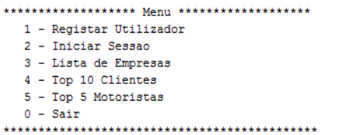
\includegraphics[width=0.7\linewidth, height=5cm]{1.png}


Opção 1 - Caso o utilizador escolha esta opção solicita o táxi mais próximo dele.

Opção 2 – Nesta opção o cliente pode solicitar um táxi especifico, podendo escolher entre carro, moto ou carrinha.

\chapter{Arquitetura da aplicação}
\section{UMERApp}

Atributos:

\begin{itemize}
    \item UMER um \par
Umer a correr na aplicação
    \item Menu\_principal \par
Menu principal.
    \item Menu menu\_registo \par
Menu de registo.
    \item Menu menu\_motorista \par
Menu para motoristas.
    \item Menu menu\_motoristaEmp \par
Menu para motoristas de empresa.
    \item Menu menu\_cliente \par
Menu para clientes.
    \item Menu menu\_solicitar \par
Menu para solicitar uma viagem.
    \item Menu menu\_veiculo \par
Menu para os tipos de veiculo
\end{itemize}

Esta classe trata de toda a interface apresentada ao utilizador, para além disso esta classe trata de gravar o estado da aplicação e ler esse mesmo quando aplicação é fechada e reiniciada. 

\subsection{Menu}
\emph{\bfseries Atributos}
\begin{itemize}
    \item List<String> opcoes \par
Lista de opções que o menu contém.
    \item int op \par
Operação escolhida pelo utilizador.
\end{itemize}

Esta classe é a classe responsável por todos os menus criados e pelo funcionamento dos mesmos. Com esta classe o trabalho da classe principal, UMERApp, é muito mais fácil.


\section{UMER}
\emph{\bfseries Atributos}

\begin{itemize}
    \item Utilizador uConectado; \par
Utilizador que está conetado na aplicação. (com sessão iniciada).
    \item CatUtilizadores catU; \par
CatUtilizadores(TreeSet<Utilizadores>) que contêm todos os utilizadores registados na Umer.
    \item CatViaturas catV; \par
CatViaturas(TreeSet<Viatura>) que contêm todos as viaturas registadas na Umer.
    \item ArrayList<Empresa> catE; \par
Lista que contêm todas as empresas existentes na Umer.
\end{itemize}

Esta classe é responsável pelo funcionamento da aplicação, é na própria que estão desenvolvidas praticamente todas as funcionalidades da nossa aplicação.

\section{Localização}
\emph{\bfseries Atributos}
\begin{itemize}
    \item int x \par
Coordenada x.
    \item int y \par
Coordenada y.
\end{itemize}
A classe Localização é responsável pela criação de uma localização (x,y) e dos cálculos de distâncias.

\section{Utilizador}
\emph{\bfseries Atributos}
\begin{itemize}
    \item String email \par
Email do Utilizador.
    \item String nome \par
Nome do Utilizador.
    \item String password \par
Password do utilizador.
    \item String morada \par
Morada do Utilizador.
    \item String dataNascimento \par
Data de nascimento do Utilizador.
    \item Localizacao local \par
Localização do Utilizador.
    \item TreeSet<Viagem> catViagens \par
Coleção de viagens efetuadas pelo Utilizador.
\end{itemize}

Classe abstrata para um utilizador, todos os utilizadores da aplicação têm em comum o que se encontra desenvolvido na própria. 

\subsection{CLiente}
Esta classe corresponde a um Cliente, esta classe herda todos os parâmetros da classe anterior.

\subsection{Motorista}
\emph{\bfseries Atributos}
\begin{itemize}
    \item int pontualidade \par
Pontualidade do motorista.
    \item int classificação \par
Classificação do motorista.
    \item long kms \par
Kilometros totais percorridos pelo motorista. 
    \item  boolean disponível \par
Disponibilidade do motorista.
    \item  ArrayList<Integer> aval \par
Lista com as avaliações do motorista feita pelos clientes.
\end{itemize}

Esta classe corresponde a um Motorista, e tal como a classe Cliente, esta classe herda os atributos da classe Utilizador aos quais são adicionados os atributos acima descritos.

\subsection{MotoristaE}
\emph{\bfseries Atributos}
\begin{itemize}
    \item Empresa empresa \par
Empresa à qual o motorista pertence.
    \item boolean disp \par
Disponibilidade do motorista.
\end{itemize}

Esta classe representa um motorista de empresa. Esta classe só tem métodos mais comuns.

\section{Empresa}
\emph{\bfseries Atributos}
\begin{itemize}
    \item long id \par
Id da Empresa.
    \item CatUtilizadores motoristas \par
TreeSet<Utilizadores> com todos os motoristas da empresa.
    \item  CatViaturas viaturas \par
TreeSet<Viaturas> com todos as viaturas da empresa.
\end{itemize}
Esta classe corresponde a uma Empresa. Esta classe só tem métodos mais comuns.

\section{Viatura}
\emph{\bfseries Atributos}
\begin{itemize}
    \item String matricula \par
Matricula da viatura.
    \item Motorista motorista \par
Motorista da viatura.
    \item double velMedia \par
Velocidade média da viatura.
    \item double custo \par
Preço por Km da viatura.
    \item double fiabilidade \par
Fiabilidade da viatura.
    \item boolean disp \par
Disponibilidade da viatura.
    \item Localizacao local; \par
Localização da viatura.
    \item   TreeSet<Viagem> catViagens; \par
Coleção de todas as viagens efetuadas pela viatura. 

\end{itemize}

Esta classe corresponde a uma Viatura. Todas as viaturas têm em comum os atributos presentes nesta classe. 

\subsection{Moto}
Esta classe corresponde a uma Viatura do tipo Moto, possuí os atributos herdados de Viatura. 

\subsection{Carro}
\emph{\bfseries Atributos}
\begin{itemize}
    \item ArrayList<Cliente> waitList; \par
Lista da fila de espera do Clientes.	
\end{itemize}
Esta classe corresponde a uma Viatura do tipo Carro, para além dos atributos herdados de Viatura, esta classe permite estabelecer uma fila de espera. 

\subsection{Carrinha}
Esta classe corresponde a uma Viatura do tipo Carrinha, possuí os atributos herdados de Viatura. 

\section{Viagem}
\emph{\bfseries Atributos}
\begin{itemize}
    \item Localizacao inicioL \par
Localização do inicio da viagem.
    \item Localizacao fimL \par
Localização do final da viagem.
    \item int classificação \par
Classificação da viagem.
    \item double tempo \par
Duração da viagem.
    \item double preco \par
Preço da viagem.
    \item Calendar inicioT \par
Data do inicio da viagem.
    \item Calendar fimT \par
Data do fim da viagem.
\end{itemize}

Esta classe corresponde a uma Viagem. Esta classe só tem métodos mais comuns. 


\chapter{Perspectivas de melhorias e trabalho futuro}

Uma aplicação deste género é sempre um produto in acabo, necessidades mudam, por isso o desenvolvimento da mesma foi feito de maneira a que uma futura alteração seja o mais fácil possível, não necessitando de refazer toda a aplicação. Um exemplo prático seria o acrescentar de um novo tipo de veiculo, bastando para tal acrescentar a sua classe e acrescentar a sua opção no menu do Motorista.  



\chapter{Conclusão}

Ao longo da realização deste trabalho fomos confrontados com algumas dificuldades, tendo sido a falta de experiencia neste novo paradigma/linguagem o maior dos obstáculos.

Mas de uma forma geral as dificuldades foram superadas, culminando num trabalho minimamente completo do qual nos podemos orgulhar e do qual retiramos conhecimento não só para realização da UC em questão, mas também para a nossa vida enquanto futuros Engenheiros Informáticos.

\end{document}
